\documentclass[useAMS,usenatbib]{mn2e}
\usepackage{footnote,graphicx,natbib,color,multirow,amsmath,url}
\voffset=-0.5in
\pdfminorversion=5
\setlength{\parsep}{0pt}
\setlength{\partopsep}{0pt}

\def\starpy ~{\textsc{starpy}}

\font\nbf=cmssbx10 at 12.28pt %big font for headers


\begin{document}


\title[Environmental quenching: yay or nay?]{Galaxy Zoo: Quenching timescales of group galaxies}
\author[Smethurst et al. 2015]{R. ~J. ~Smethurst,$^{1}$ C. ~J. ~Lintott,$^{1}$ and the Galaxy Zoo team \footnotemark[1]
\\ $^1$ Oxford Astrophysics, Department of Physics, University of Oxford, Denys Wilkinson Building, Keble Road, Oxford, OX1 3RH, UK 
}

\maketitle

\begin{abstract}
Does the environment of a galaxy directly influence the quenching timescale of a galaxy? Here we construct a sample of group and field galaxies with morphological classifications from Galaxy Zoo 2 and use Bayesian inference to determine the quenching time and exponential timescale that describes a simple SFH for a given galaxy from its photometry. We observe how the detailed morphological structures, such as bars and bulges, are affected by environment and correlate this with changes in the quenching timescales. Mass quenching is seen to be just as important for satellite galaxies as central galaxies.  We find that the environment does play a direct role in galaxy quenching through a mechanism which is correlated to the halo mass of a group. It is not correlated with the relative velocity of satellite galaxies within the group, therefore mechanisms such as ram pressure stripping are not the main cause of quenching in the group environment. 

\end{abstract}

\begin{keywords}
galaxies -- environment, galaxies -- photometry, galaxies -- statistics, galaxies -- morphology
\end{keywords}

\footnotetext[1]{This investigation has been made possible by the participation of over 350,000 users in the Galaxy Zoo project. Their contributions are acknowledged at \url{http://authors.galaxyzoo.org}}

\section{Introduction}\label{sec:intro}
 
 There are many mechanisms which are proposed to cause quenching; including mergers \citep{daddi10}, mass quenching \citep{kennicutt77, peng12}, morphological quenching \citep{faber12} and the environment of a galaxy.
 
 The galaxy environment as a cause of quenching was proposed due to the correlation of both morphology \citep{dressler80} and the quenched galaxy fraction \citep{?} with environmental density. However, does this correlation truly imply causation? Evidence from simulations \citep{?} suggests that the environment may not be the dominant quenching mechanism in the galaxy lifecycle. Perhaps the correlation of increased galaxy quenched fractions with environment is due to a superposition of the effects of mergers, interactions and both mass \& morphology quenching. In denser environments, galaxies are more likely to encounter another galaxy in a merger or interaction scenario and infall over long timescales during which gas reservoirs can be depleted due to star formation via mass quenching.
 
There has been mounting evidence that the oft proposed mechanism behind environmental quenching - ram pressure stripping \citep{?} - may not be effective at quenching as first thought \citep{}. 
 
In order to isolate the case of the density-morphology and density-SFR correlations, we need to study how galaxy quenching timescales and morphology change in group and field environments with different properties. To do this we construct a sample of both group and field galaxies and utilise Bayesian inference to determine the quenching time and exponential timescale to describe a simple SFH for a galaxy given its photometry. We aim to determine the following: (i) How does the environment influence the detailed morphological structures of a galaxy?  (ii) Does the environment directly cause quenching? (iii) If so, what environmental mechanism is responsible for this quenching?

In Section~\ref{sec:data} we describe our data sources and inference methods and highlight our results in Section~\ref{sec:results}. We then discuss these results and how they fit into the bigger picture of quenching in Section~\ref{sec:disc}. The zero points of all magnitudes are in the AB system. Where necessary, we adopt the WMAP Seven-Year Cosmology \citep{jarosik11} with $(\Omega_m , ~\Omega_\Lambda , ~h) = (0.26, 0.73, 0.71)$.

 
\section{Data and Methods}\label{sec:data}

\subsection{Data Sources}\label{sec:photo}

In this investigation we use visual classifications of galaxy morphologies from the Galaxy Zoo 2\footnote{\url{http://zoo2.galaxyzoo.org/}} (GZ2) citizen science project \citep{GZ2}, which obtains multiple independent classifications for each optical image. The full question tree for an image is shown in Figure~1 of \citeauthor{GZ2}  The GZ2 project used $304, 022$ images from the Sloan Digital Sky Survey Data Release 7 (SDSS; \citealt{york00, abazajian09}) all classified by \emph{at least} 17 independent users, with a mean number of classifications of $\sim42$.

Further to this, we required NUV photometry from the GALEX survey \citep{martin05}, within which $\sim42\%$ of the GZ2 sample was observed, giving $126, 316$ galaxies total ($0.01 < z < 0.25$). This will be referred to as the \textsc{gz2-galex} sample. The completeness of this sample ($-22 < M_u < -15$) is shown in Figure~2 of \cite{smethurst15}. 

Observed fluxes are corrected for galactic extinction \citep{Oh11} by applying the \citet{cardelli89} law. We also adopt $k$-corrections to $z = 0.0$ and obtain absolute magnitudes from the NYU-VAGC \citep{blanton05, blanton07, padmanabhan08}.

\begin{figure*}
\centering{
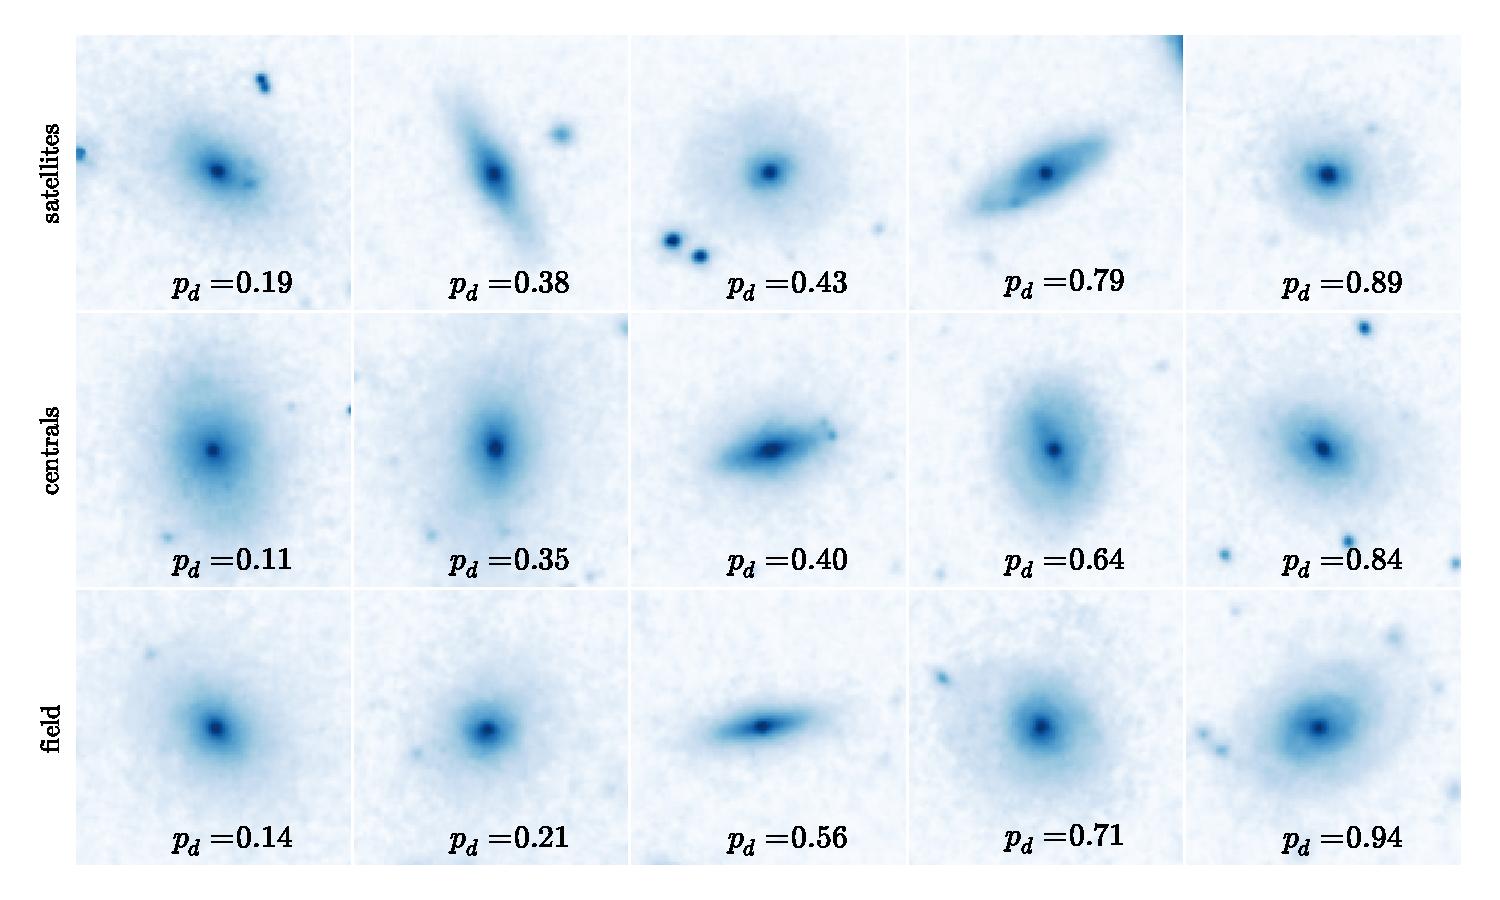
\includegraphics[width=0.95\textwidth]{mosaic_sat_cent_field_disc_fraction.pdf}
\caption{Randomly selected SDSS \emph{gri} composite images of satellite and central galaxies in the \textsc{gz2-group} sample in comparison to those from the \textsc{gz2-field} sample. All galaxies lie within $0.04 < z < 0.05$ and in the central galaxy mass range $10^{10.5} < M_{*} [M_{\odot}] < 10^{11}$, used as a proxy for halo mass. The galaxies are ordered from least to most featured according to their debiased `disc or featured' vote fraction, $p_d$ (see \citealt{willett13}). The scale for each image is $0.099~\rm{arcsec/pixel}$.}}
\label{fig:mosaic}
\end{figure*}

\subsection{Group Identification}\label{sec:groups}



We used the \citet{berlind06} catalogue, which uses a friends-of-friends algorithm to identify group and cluster galaxies in the SDSS. This was cross matched to the \textsc{gz2-galex} sample and limited to $z < 0.1$ to ensure GALEX completeness of the red sequence (see \citealt{wyder07, yesuf14}). Centrals were selected as the most massive galaxy in a group and all others were designated as satellites (masses were calculated using the absolute r-band magnitude and $u-r$ colour and the method of \citealt{baldry06}). This resulted in a sample of $14,199$ group galaxies with $3,468$ centrals and $10,731$ satellites within a projected cluster centric radius range of $0 < R/R_{200} < 25$ and $z < 0.084$. 

In this work we focus on galaxies which are either quenching or quenched and are more than $\pm1\sigma$ below the star forming `main sequence'. This encompasses $4629$ satellite and $2314$ central galaxies and will be referred to as the \textsc{gz2-group} sample. These galaxies are highlighted in red on Figure \ref{}. 

\subsection{Field sample}\label{sec:field}

For all galaxies in the \textsc{gz-galex} sample, we calculated the smallest projected cluster centric radii from each of the central galaxies in the  \citet{berlind06} catalog and selected candidate field galaxies as those with (i) $R/R_{200} > 25$ and (ii) $\log\Sigma < -0.8$ from \cite{baldry06}. This sample of field galaxy candidates was then matched in redshift and stellar mass firstly to the central galaxies of the \textsc{gz2-group} sample to give $2,309$ field galaxies with $z < 0.084$ which will be referred to as the \textsc{gz2-cent-field} sample. Secondly, the field galaxy candidates were then matched in redshift and stellar mass to the satellite galaxies of the \textsc{gz2-group} sample to give $6,849$ field galaxies with $z < 0.084$ which will be referred to as the \textsc{gz2-sat-field}. These galaxies in the \textsc{gz2-sat-field} sample will be used as a control when investigating the morphological trends of satellite galaxies with environment. 

As in Section \ref{sec:groups} we select all those galaxies in the central matched sample $\pm1\sigma$ below the star forming `main sequence', giving $1596$ quenching or quenched field galaxies for use as a control sample, which will be referred to as the \textsc{gz2-cent-field-q} sample. These galaxies will be used as a control when investigating the quenching parameters of the different environments in order to ensure that each galaxy under comparison resides in similar stellar mass halos. 
%We also select all those galaxies in the satellite matched sample $\pm1\sigma$ below the star forming `main sequence', giving $$ quenching or quenched field galaxies for use as a control sample, which will be referred to as the \textsc{gz2-sat-field-q} sample.
  

\begin{figure}
\centering{
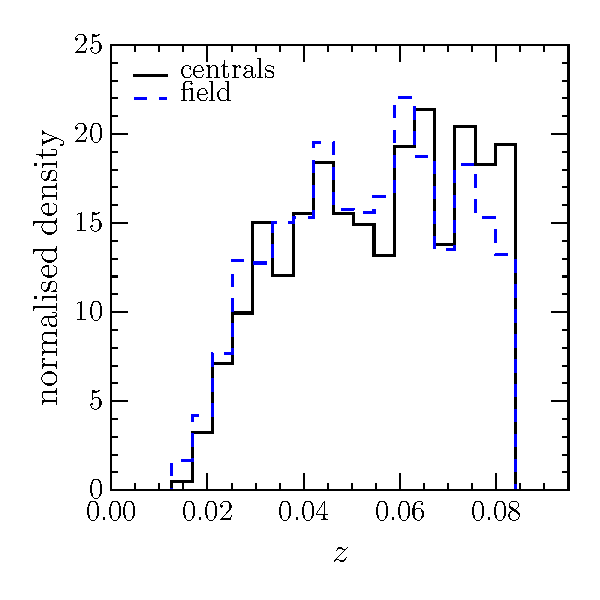
\includegraphics[width=0.45\textwidth]{redshift_cent_field.pdf}
\caption{Redshift distributions of quenching or quenched central galaxies in the \textsc{gz2-group} sample (black solid line) in comparison to the redshift and mass matched \textsc{gz2-cent-field-q} sample (blue dashed line).}}
\label{fig:zcompare}
\end{figure}

\subsection{Deriving quenching parameters}\label{sec:starpy}

\textsc{starpy}\footnote{Publicly available: \url{http://github.com/zooniverse/starpy}} is a \textsc{python} code which allows the user to derive the quenching star formation history (SFH) of a single galaxy through a Bayesian Markov Chain Monte Carlo method \citep{emcee13}\footnote{\url{http://dan.iel.fm/emcee/}} with the input of the observed $u-r$ and $NUV-u$ colours, a redshift, and the use of the stellar population models of \cite{BC03}.  These models are implemented using solar metallicity (varying this does not substantially affect these results; \citealt{smethurst15}) and a Chabrier IMF \citep{Chab03} but does not model for intrinsic dust. The SFH is modelled as an exponential decline of the SFR described by two parameters $[t_{q}, \tau]$, where $t_{q}$ is the time at the onset of quenching $\rm{[Gyr]}$ and $\tau$ is the exponential rate at which quenching occurs $\rm{[Gyr]}$. Under the simplifying assumption that all galaxies formed at $t=0$ $\rm{ Gyr}$ with an initial burst of star formation, the SFH can be described as: 
\begin{equation}\label{sfh}
SFR =
\begin{cases}
i_{sfr}(t_{q}) & \text{if } t < t_{q} \\
i_{sfr}(t_{q}) \times exp{\left( \frac{-(t-t_{q})}{\tau}\right)} & \text{if } t > t_{q} 
\end{cases}
\end{equation}
where $i_{sfr}$ is an initial constant star formation rate dependent on $t_{q}$ \citep{schawinski14, smethurst15}.  A smaller $\tau$ value corresponds to a rapid quench, whereas a larger $\tau$ value corresponds to a slower quench. We note that a galaxy undergoing a slow quench is not necessarily quiescent by the time of observation. Similarly, despite a rapid quenching rate, star formation in a galaxy may still be ongoing at very low rates, rather than being fully quenched. This SFH model has previously been shown to appropriately characterise quenching galaxies \citep{Weiner06, Martin07, Noeske07,schawinski14}. We note also that star forming galaxies in this regime are fit by a constant SFR with a $t_{q} \simeq$ Age$(z)$, (i.e. the age of the Universe at the galaxy's observed redshift) with a very low probability.

The probabilistic fitting methods to these star formation histories for an observed galaxy are described in full detail in Section 3.2 of \cite{smethurst15}, wherein the \starpy ~~code was used to characterise the SFHs of each galaxy in the \textsc{gz2-galex} sample. We assume a flat prior on all the model parameters and the difference between the observed and predicted $u-r$ and $NUV-u$ colours are modelled as independent realisations of a double Gaussian likelihood function (Equation 2 in \citealt{smethurst15}). We also make the simplifying assumption that the age of each galaxy, $t_\mathrm{age}$ corresponds to the age of the Universe at its observed redshift, $t_\mathrm{obs}$.

The output of \starpy  ~ is probabilistic in nature and provides the posterior probability distribution across the two-parameter space for an individual galaxy the degeneracies for which can be seen in Figure~4 of \citet{smethurst15}. We take the 50th percentile walker position of these individual posterior probability distributions to give the most likely $t_{q}$ and $\tau$ for each galaxy. 

In this work we will look for trends in the time since quenching onset, $\Delta t$, for a given galaxy by calculating $\Delta t = t_\mathrm{obs} - t_{q}$. We will observe how this quantity changes with group properties such as halo mass (here we use the stellar mass of the group central as a proxy for halo mass), velocity dispersion and the number of group members. 

\section{Results}\label{sec:results}

\begin{figure}
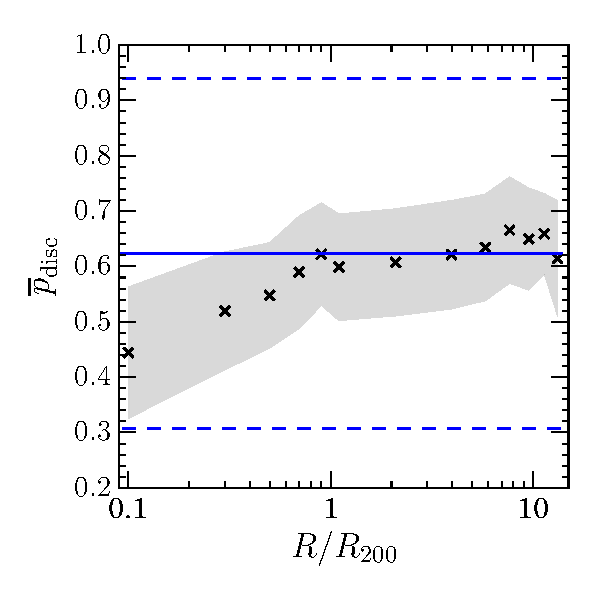
\includegraphics[width=0.46\textwidth]{p_disc_trend_with_log_radius_field_compare.pdf}
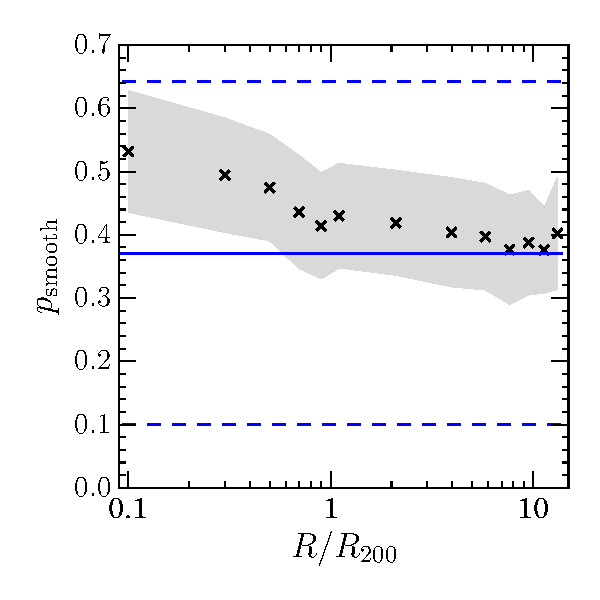
\includegraphics[width=0.46\textwidth]{p_smooth_trend_with_log_radius_field_compare.pdf}
\caption{Mean GZ vote fraction for disc (top) and smooth (bottom) galaxies in the \textsc{gz2-group} sample binned in projected cluster centric radius, normalised by $R_{200}$, a proxy for the virial radius of a group. The shaded region shows $\pm1\sigma$ on the mean vote fraction. The mean vote fraction of the \textsc{field} sample are also shown (blue solid lines) with $\pm1\sigma$ (blue dashed lines).}
\label{fig:morphradius}
\end{figure}

\begin{figure}
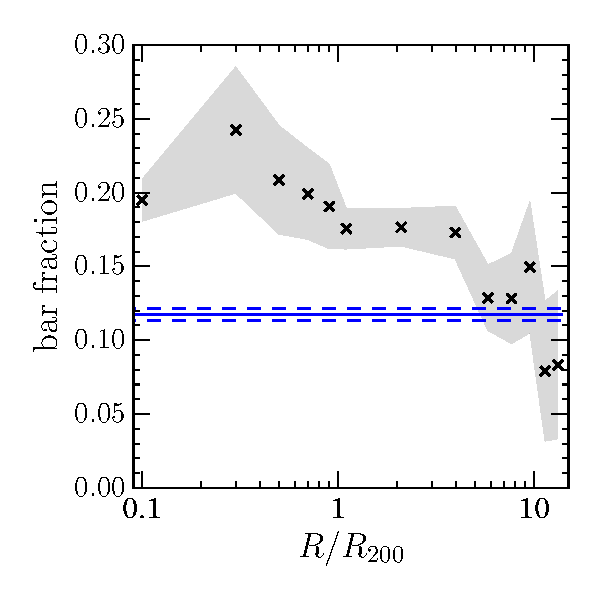
\includegraphics[width=0.46\textwidth]{bar_fraction_over_disc_trend_with_log_radius_sat_matched_field_cand.pdf}
\caption{Bar fraction (number of barred disc galaxies over number of disc galaxies) in the \textsc{gz2-group} sample binned in projected cluster centric radius, normalised by $R_{200}$, a proxy for the virial radius of a group. The shaded region shows $\pm1\sigma$ on the bar fraction. The bar fraction of the \textsc{gz2-sat-field} sample is also shown (blue solid line) with $\pm1\sigma$ (blue dashed line).}
\label{fig:barradius}
\end{figure}

\begin{figure}
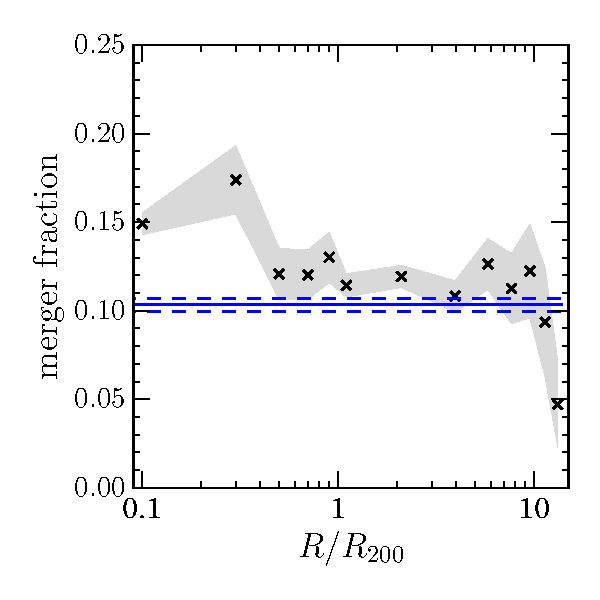
\includegraphics[width=0.46\textwidth]{merger_fraction_trend_with_log_radius_compare_sat_field_cand.pdf}
\caption{Merger fraction in the \textsc{gz2-group} sample binned in projected cluster centric radius, normalised by $R_{200}$, a proxy for the virial radius of a group. The shaded region shows $\pm1\sigma$ on the merger fraction. The merger fraction of the \textsc{gz2-sat-field} sample is also shown (blue solid line) with $\pm1\sigma$ (blue dashed line).}
\label{fig:mergerradius}
\end{figure}

First start with a sanity check - do we reproduce morphology-density relation of \citealt{dressler80}? Figure \ref{fig:morphradius} shows the mean disc and smooth vote fractions from galaxy zoo, binned in projected cluster centric radius (normalised by the approximate viral radius of each group, $R_{200}$). We can see that the mean disc (smooth) vote fraction decreases (increases) from the mean field value (blue line) past $1$ virial radius.

Figure \ref{fig:barradius} shows how the bar fraction (number of barred disc galaxies over the number of disc galaxies) increases towards the centre of the group population suggesting the possibility that the environment may play a role in triggering the disk instabilities which produce a morphological bar \citep{ref, ref, ref}. 

Figure \ref{fig:mergerradius} shows how the merger fraction does not significantly deviate from the field fraction (blue line) until beyond $1$ virial radius. Similarly in Figure \ref{fig:bulgeradius} the left panel shows how those galaxies identified as having no or just noticeable bulges are less common in the inner regions of the cluster (left panel), whereas the fraction of galaxies with obvious or dominant bulges (thought to be grown by mergers;\citealt{ref, ref, ref}) increases with decreasing projected distance from the centre of the cluster 

Figure \ref{fig:sfrradius} shows how the SFR of the \textsc{gz2-group} sample declines with decreasing cluster centric distance, significantly below the mean SFR of the \textsc{gz2-field} sample shown by the blue dashed line. This is in agreement with the results of \cite{gomez03} who observe the decline in SFR with cluster centric radius in SDSS clusters (see for example, Figure 6 in \citealt{gomez03}). 

With the results from \starpy~ we can look at the time since quenching onset ($\Delta t = t_{obs} - t_{q}$, see Section \ref{}) binned in projected cluster centric radius, normalised by $R_{200}$ (a proxy for virial radius) for satellite galaxies and central galaxies in the \textsc{gz2-group} sample, compared with galaxies in the \textsc{gz2-field} sample. We can investigate these trends with group properties as shown in Figures \ref{fig:timesinceradius} \& \ref{fig:timesinceradiusvel}. 

If mergers are an important evolutionary mechanism for satellite galaxies, we expect to see a difference in the quenching histories of satellites in groups with a higher number of galaxies, $N_{group}$. However, if we look at the bottom panel of Figure \ref{fig:timesinceradius} we do not see a trend with time since quenching onset with increasing $N_{group}$ for the satellite galaxies. The only place we do see such a trend for the central galaxies. 

Across all the panels in Figures \ref{fig:timesinceradius} \& \ref{fig:timesinceradiusvel} we see a general trend for increasing time since quench with decreasing distance from the centre, which is suggestive that this slight trend is due to an effect of the environment itself. As earlier, in Figures \ref{fig:morphradius}$-$\ref{fig:bulgeradius} significant differences from the field value arise beyond approximately one virial radius. 

In the middle panel of Figure \ref{fig:timesinceradius} however, we do see a clear trend for increasing time since quenching onset with increasing stellar mass for both satellite and central galaxies. This is suggestive of mass quenching among the group galaxy population. This is contrary to previous work suggesting that mass quenching is only of import for central galaxies \citep{ref, ref, ref}. 

In simulations, the three things that are seen to constrain galaxy evolution are redshift, mass and halo mass \cite{ref, ref}. To study the effect that halo mass has on the quenching properties of group galaxies we shall use a proxy for halo mass by splitting by the mass of the corresponding central galaxy of the group.

We investigate the effect of the group halo mass in the top panel of Figure \ref{fig:timesinceradius} where we can once again see a clear trend for increasing time since quenching onset with increasing stellar mass of the group central for both satellite and central galaxies. More massive halos therefore have a greater impact on the star formation rate of their satellites than less massive halos. 

In the bottom panel of Figure \ref{fig:timesinceradiusvel} we split the satellite galaxies of the \textsc{gz2-group} sample into bins of relative velocity to their central galaxies. We can see that their is no trend with time since onset of quenching with increasing relative velocity for satellite galaxies, however the trend with decreasing projected group centric radius, seen in each panel in Figure \ref{fig:timesinceradius} is still present. This suggests that any environmental processes causing this quenching are not corrected with satellite velocity.  

\begin{figure*}
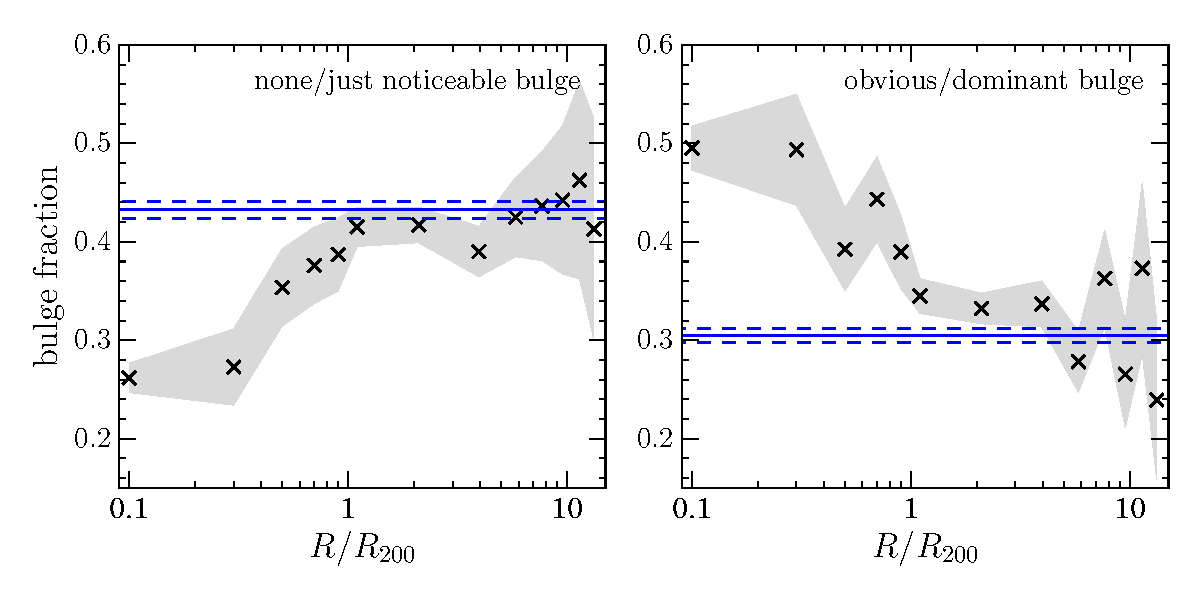
\includegraphics[width=0.85\textwidth]{min_max_bulge_fraction_trend_with_log_radius_sat_field_cand.pdf}
\caption{Fraction of galaxies with none/just noticeable bulge classifications (left) and with obvious/dominant bulge classifications (right) in the \textsc{gz2-group} sample binned in projected cluster centric radius, normalised by $R_{200}$, a proxy for the virial radius of a group. The shaded regions shows $\pm1\sigma$ on the bulge fractions. The bulge fractions of the \textsc{gz2-sat-field} sample are also shown (blue solid lines) with $\pm1\sigma$ (blue dashed lines).}
\label{fig:bulgeradius}
\end{figure*}

\begin{figure}
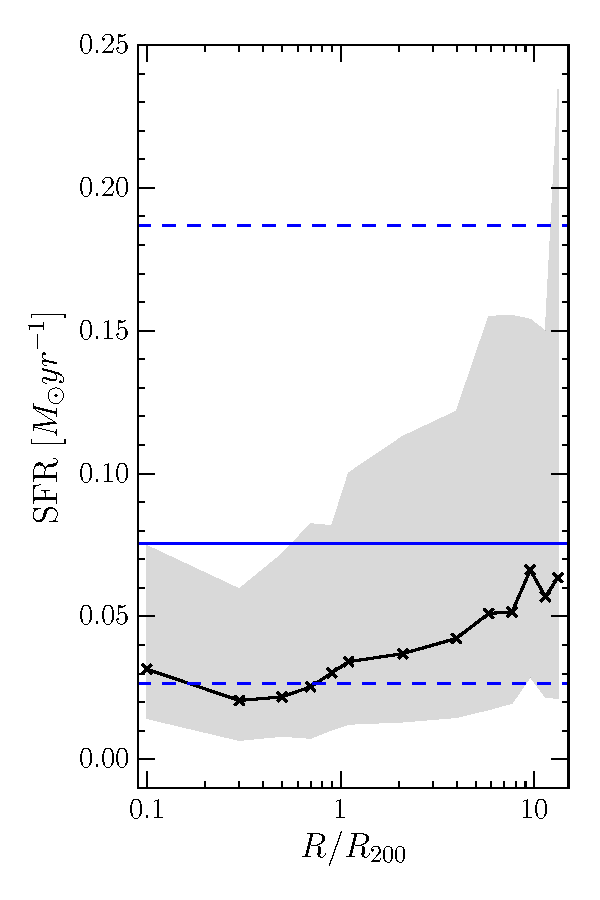
\includegraphics[width=0.46\textwidth]{sfr_trend_with_log_radius_field_matched_blue_dashed_hlines_gomez_03_rv_not_r200.pdf}
\caption{Median $H\alpha$ derived star formation rates of satellite galaxies in the \textsc{gz2-group} sample, binned in projected cluster centric radius, normalised by $R_{200}$, a proxy for the virial radius of a group.  The shaded region shows the SFRs encompassed by $50\%$ of the population in a given bin. The median SFR of the \textsc{gz2-sat-field} sample is shown (blue solid line) along with the 25th and 75th percentiles (blue dashed lines).}
\label{fig:sfrradius}
\end{figure}

\begin{figure}
\centering{
\includegraphics[height=0.875\textheight]{time_since_quenching_environment_properties.pdf}
\caption{The time since quenching onset ($\Delta t = t_{obs} - t_{q}$) binned in projected cluster centric radius, normalised by $R_{200}$, for satellite galaxies (triangles) split by stellar mass of the corresponding central galaxy (top), stellar mass (middle) and the number of galaxies within the group (bottom). The corresponding values for central galaxies (squares) and galaxies in the \textsc{gz2-cent-field} sample (circles) are shown and connected by the dashed lines to aid the reader.}
\label{fig:timesinceradius}}
\end{figure}

\begin{figure}
\centering{
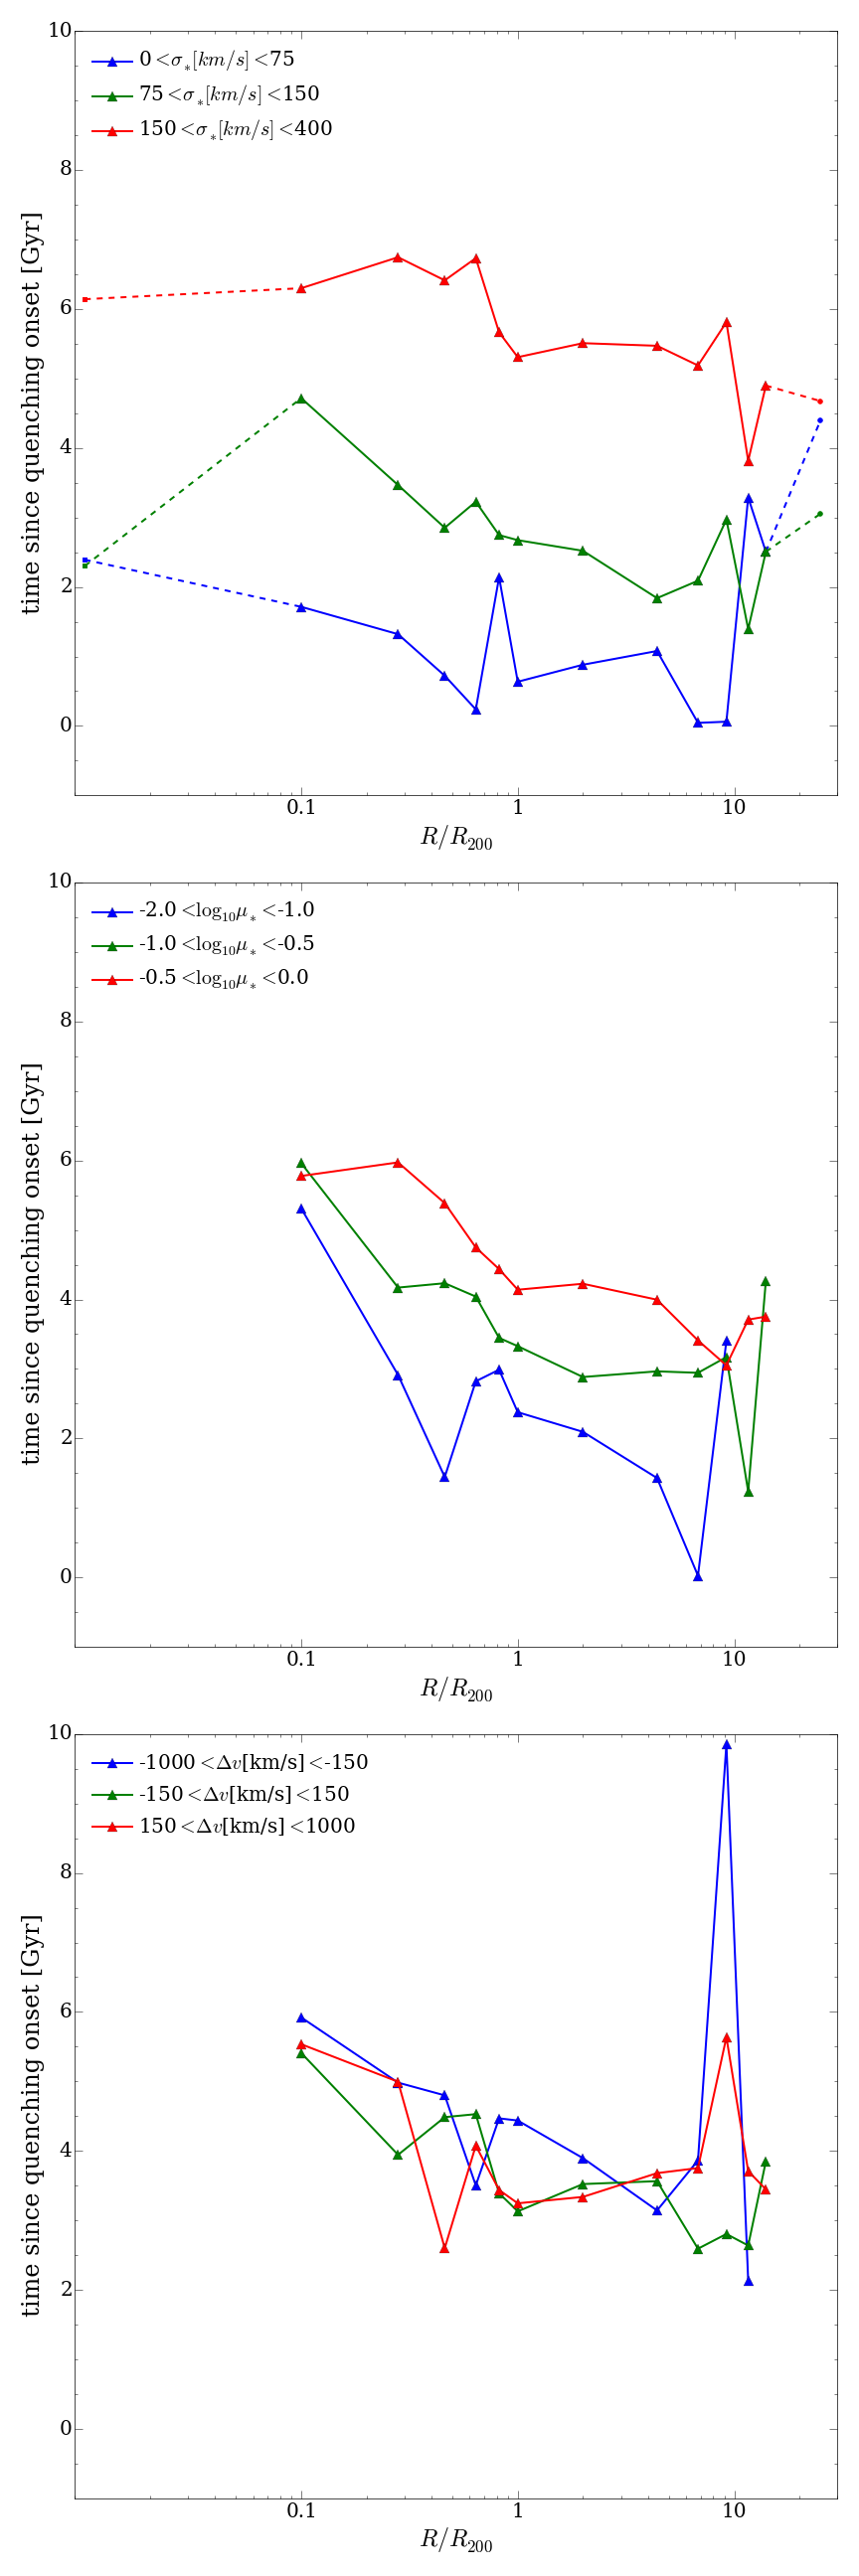
\includegraphics[height=0.875\textheight]{time_since_quenching_v_disp_mu_bins_delv.pdf}
\caption{The time since quenching onset ($\Delta t = t_{obs} - t_{q}$) binned in projected cluster centric radius, normalised by $R_{200}$, for satellite galaxies (triangles) split by velocity dispersion (top), stellar mass ratio ($\mu_* = M_*/M_{*,c}$) (middle) and the difference in velocity from the associated central galaxy (bottom). The corresponding values for central galaxies (squares) and galaxies in the \textsc{gz2-cent-field} sample (circles) are shown and connected by the dashed lines to aid the reader in the top panel where appropriate.}
\label{fig:timesinceradiusvel}}
\end{figure}


\section{Discussion}\label{sec:disc}

We have shown that mergers are important for centrals not for satellites in the bottom panel of Figure \ref{fig:timesinceradius}, that mass quenching is important for satellites as well as centrals in the middle panel of Figure \ref{fig:timesinceradius} and that larger halos have a stronger environmental effect on their satellites in the top panel of Figure \ref{fig:timesinceradius}. 

The trend that is present in all panels of Figure \ref{fig:timesinceradius} was for increasing time since quenching onset with decreasing projected group centric distance. We argue that this lends more support for quenching caused directly by the environmental; galaxies closer in, fell into the group earlier, as they did so they started quenching and so have a longer time since quenching started to occur. However, as seen in Figure \ref{fig:timesinceradiusvel} there is no trend in the time since quenching onset with the relative velocity of the satellites to their corresponding central. This suggests that whatever environmental mechanism is at play here, it is dependant on the size of the halo, either due to the potential or temperature of the halo, but not dependant on the speed of the satellite as in ram pressure stripping theory. This suggests that ram pressure stripping is not the dominant environmental quenching mechanism. 

\subsection{The Big Picture}\label{sec:bigpic}

\section{Conclusions}\label{sec:conc}

Mass quenching is definitely prevalent for satellites and mergers are important only in the most inner regions of groups for central galaxies. The environment does play a role in quenching galaxies through a mechanism proportional to the halo mass of the group but which isn't proportional to the speed the satellite galaxy is moving at relative to it's central galaxy. This suggests that ram pressure stripping is therefore not the dominant mechanism at work in environmental quenching. 



\bibliographystyle{mn2e}
\bibliography{refs}  

\end{document}